\documentclass[12pt,twoside]{article}
\usepackage[dvipsnames]{xcolor}
\usepackage{tikz,graphicx,amsmath,amsfonts,amscd,amssymb,bm,cite,epsfig,epsf,url}
\usepackage[hang,flushmargin]{footmisc}
\usepackage[colorlinks=true,urlcolor=blue,citecolor=blue]{hyperref}
\usepackage{amsthm,multirow,wasysym,appendix}
\usepackage{array,subcaption} 
% \usepackage[small,bf]{caption}
\usepackage{bbm}
\usepackage{pgfplots}
\usetikzlibrary{spy}
\usepgfplotslibrary{external}
\usepgfplotslibrary{fillbetween}
\usetikzlibrary{arrows,automata}
\usepackage{graphicx}
\usepackage{thmtools}
\usepackage{blkarray} 
\usepackage{textcomp}
\newcommand{\red}[1]{{\leavevmode\color{red}{#1}}}
\newcommand{\blue}[1]{{\leavevmode\color{blue}{#1}}}
\usepackage[left=0.8in,right=1.0in,top=1.0in,bottom=1.0in]{geometry}

%% Probability operators and functions
%
% \def \P{\mathrm{P}}
\def \P{\mathrm{P}}
\def \E{\mathrm{E}}
\def \Var{\mathrm{Var}}
\let\var\Var
\def \Cov {\mathrm{Cov}} \let\cov\Cov
\def \MSE {\mathrm{MSE}} \let\mse\MSE
\def \sgn {\mathrm{sgn}}
\def \R {\mathbb{R}}
\def \C {\mathbb{C}}
\def \N {\mathbb{N}}
\def \Z {\mathbb{Z}}
\def \cV {\mathcal{V}}
\def \cS {\mathcal{S}}

\newcommand{\RR}{\ensuremath{\mathbb{R}}}

\DeclareMathOperator*{\argmin}{arg\,min}
\DeclareMathOperator*{\argmax}{arg\,max}
\newcommand{\red}[1]{\textcolor{red}{#1}}
\newcommand{\blue}[1]{\textcolor{blue}{#1}}
\newcommand{\green}[1]{\textcolor{ForestGreen}{ #1}}
\newcommand{\fuchsia}[1]{\textcolor{RoyalPurple}{ #1}}

\newcommand{\wrnd}[1]{\widetilde{ #1 } }
\newcommand{\po}{\wrnd{\op{po}}  }

%
%% Probability distributions
%
%\def \Bern    {\mathrm{Bern}}
%\def \Binom   {\mathrm{Binom}}
%\def \Exp     {\mathrm{Exp}}
%\def \Geom    {\mathrm{Geom}}
% \def \Norm    {\mathcal{N}}
%\def \Poisson {\mathrm{Poisson}}
%\def \Unif    {\mathrm {U}}
%
\DeclareMathOperator{\Norm}{\mathcal{N}}

\newcommand{\bdb}[1]{\textcolor{red}{#1}}

\newcommand{\ml}[1]{\mathcal{ #1 } }
\newcommand{\wh}[1]{\widehat{ #1 } }
\newcommand{\wt}[1]{\widetilde{ #1 } }
\newcommand{\conj}[1]{\overline{ #1 } }
\newcommand{\rnd}[1]{\tilde{ #1 } }
\newcommand{\rv}[1]{ \rnd{ #1}  }
\newcommand{\rM}{\rnd{ m}  }
\newcommand{\rx}{\rnd{ x}  }
\newcommand{\ry}{\rnd{ y}  }
\newcommand{\rz}{\rnd{ z}  }
\newcommand{\ra}{\rnd{ a}  }
\newcommand{\rb}{\rnd{ b}  }
\newcommand{\rt}{\rnd{ t}  }
\newcommand{\rs}{\rnd{ s}  }


\newcommand{\rpc}{\widetilde{ pc}  }
\newcommand{\rndvec}[1]{\vec{\rnd{#1}}}

\def \cnd {\, | \,}
\def \Id { I }
\def \J {\mathbf{1}\mathbf{1}^T}

\newcommand{\op}[1]{\operatorname{#1}}
\newcommand{\setdef}[2]{ := \keys{ #1 \; | \; #2 } }
\newcommand{\set}[2]{ \keys{ #1 \; | \; #2 } }
\newcommand{\sign}[1]{\op{sign}\left( #1 \right) }
\newcommand{\trace}[1]{\op{tr}\left( #1 \right) }
\newcommand{\tr}[1]{\op{tr}\left( #1 \right) }
\newcommand{\inv}[1]{\left( #1 \right)^{-1} }
\newcommand{\abs}[1]{\left| #1 \right|}
\newcommand{\sabs}[1]{| #1 |}
\newcommand{\keys}[1]{\left\{ #1 \right\}}
\newcommand{\sqbr}[1]{\left[ #1 \right]}
\newcommand{\sbrac}[1]{ ( #1 ) }
\newcommand{\brac}[1]{\left( #1 \right) }
\newcommand{\bbrac}[1]{\big( #1 \big) }
\newcommand{\Bbrac}[1]{\Big( #1 \Big)}
\newcommand{\BBbrac}[1]{\BIG( #1 \Big)}
\newcommand{\MAT}[1]{\begin{bmatrix} #1 \end{bmatrix}}
\newcommand{\sMAT}[1]{\left(\begin{smallmatrix} #1 \end{smallmatrix}\right)}
\newcommand{\sMATn}[1]{\begin{smallmatrix} #1 \end{smallmatrix}}
\newcommand{\PROD}[2]{\left \langle #1, #2\right \rangle}
\newcommand{\PRODs}[2]{\langle #1, #2 \rangle}
\newcommand{\der}[2]{\frac{\text{d}#2}{\text{d}#1}}
\newcommand{\pder}[2]{\frac{\partial#2}{\partial#1}}
\newcommand{\derTwo}[2]{\frac{\text{d}^2#2}{\text{d}#1^2}}
\newcommand{\ceil}[1]{\lceil #1 \rceil}
\newcommand{\Imag}[1]{\op{Im}\brac{ #1 }}
\newcommand{\Real}[1]{\op{Re}\brac{ #1 }}
\newcommand{\norm}[1]{\left|\left| #1 \right|\right| }
\newcommand{\norms}[1]{ \| #1 \|  }
\newcommand{\normProd}[1]{\left|\left| #1 \right|\right| _{\PROD{\cdot}{\cdot}} }
\newcommand{\normTwo}[1]{\left|\left| #1 \right|\right| _{2} }
\newcommand{\normTwos}[1]{ \| #1  \| _{2} }
\newcommand{\normZero}[1]{\left|\left| #1 \right|\right| _{0} }
\newcommand{\normTV}[1]{\left|\left| #1 \right|\right|  _{ \op{TV}  } }% _{\op{c} \ell_1} }
\newcommand{\normOne}[1]{\left|\left| #1 \right|\right| _{1} }
\newcommand{\normOnes}[1]{\| #1 \| _{1} }
\newcommand{\normOneTwo}[1]{\left|\left| #1 \right|\right| _{1,2} }
\newcommand{\normF}[1]{\left|\left| #1 \right|\right| _{\op{F}} }
\newcommand{\normLTwo}[1]{\left|\left| #1 \right|\right| _{\ml{L}_2} }
\newcommand{\normNuc}[1]{\left|\left| #1 \right|\right| _{\ast} }
\newcommand{\normOp}[1]{\left|\left| #1 \right|\right|  }
\newcommand{\normInf}[1]{\left|\left| #1 \right|\right| _{\infty}  }
\newcommand{\proj}[1]{\mathcal{P}_{#1} \, }
\newcommand{\diff}[1]{ \, \text{d}#1 }
\newcommand{\vc}[1]{\boldsymbol{\vec{#1}}}
\newcommand{\rc}[1]{\boldsymbol{#1}}
\newcommand{\vx}{\vec{x}}
\newcommand{\vy}{\vec{y}}
\newcommand{\vz}{\vec{z}}
\newcommand{\vu}{\vec{u}}
\newcommand{\vv}{\vec{v}}
\newcommand{\vb}{\vec{\beta}}
\newcommand{\va}{\vec{\alpha}}
\newcommand{\vaa}{\vec{a}}
\newcommand{\vbb}{\vec{b}}
\newcommand{\vg}{\vec{g}}
\newcommand{\vw}{\vec{w}}
\newcommand{\vh}{\vec{h}}
\newcommand{\vbeta}{\vec{\beta}}
\newcommand{\valpha}{\vec{\alpha}}
\newcommand{\vgamma}{\vec{\gamma}}
\newcommand{\veta}{\vec{\eta}}
\newcommand{\vnu}{\vec{\nu}}
\newcommand{\rw}{\rnd{w}}
\newcommand{\rvnu}{\vc{\nu}}
\newcommand{\rvv}{\rndvec{v}}
\newcommand{\rvw}{\rndvec{w}}
\newcommand{\rvx}{\rndvec{x}}
\newcommand{\rvy}{\rndvec{y}}
\newcommand{\rvz}{\rndvec{z}}
\newcommand{\rvX}{\rndvec{X}}


\newtheorem{theorem}{Theorem}[section]
% \declaretheorem[style=plain,qed=$\square$]{theorem}
\newtheorem{corollary}[theorem]{Corollary}
\newtheorem{definition}[theorem]{Definition}
\newtheorem{lemma}[theorem]{Lemma}
\newtheorem{remark}[theorem]{Remark}
\newtheorem{algorithm}[theorem]{Algorithm}

% \theoremstyle{definition}
%\newtheorem{example}[proof]{Example}
\declaretheorem[style=definition,qed=$\triangle$,sibling=definition]{example}
\declaretheorem[style=definition,qed=$\bigcirc$,sibling=definition]{application}

%
%% Typographic tweaks and miscellaneous
%\newcommand{\sfrac}[2]{\mbox{\small$\displaystyle\frac{#1}{#2}$}}
%\newcommand{\suchthat}{\kern0.1em{:}\kern0.3em}
%\newcommand{\qqquad}{\kern3em}
%\newcommand{\cond}{\,|\,}
%\def\Matlab{\textsc{Matlab}}
%\newcommand{\displayskip}[1]{\abovedisplayskip #1\belowdisplayskip #1}
%\newcommand{\term}[1]{\emph{#1}}
%\renewcommand{\implies}{\;\Rightarrow\;}



\begin{document}

\begin{center}
{\large{\textbf{Homework 1}} } \vspace{0.2cm}\\
Due September 18 at 11 pm
\\
\end{center}
Unless stated otherwise, justify any answers you give.
You can work in groups, but each
student must write their own solution based on their own
understanding of the problem.

When uploading your homework to Gradescope you will have to
select the relevant pages for each question.  Please submit each
problem on a separate page (i.e., 1a and~1b can be on the same page but 1
and 2 must be on different pages).  We understand that this may be
cumbersome but this is the best way for the grading team to grade your
homework assignments and provide feedback in a timely manner.  Failure
to adhere to these guidelines may result in a loss of points.
Note that it may take some time to
select the pages for your submission.  Please plan accordingly.  We
suggest uploading your assignment at least 30 minutes before the deadline
so you will have ample time to select the correct pages for your
submission.  If you are using \LaTeX, consider using the minted or
listings packages for typesetting code.  
\\

\begin{enumerate}

\item (True or False)
Prove the following statements or provide a counterexample. Let $A$, $B$, and $C$ be events in a probability space.
\begin{enumerate}
\item If $A$ and $B$ are independent, then so are $A^c$ and $B$.
\blue{
\begin{itemize}
    \item by the law of total probability we know $P(B)=P(A\cap B)+P(A^c\cap B)$ since A and $A^c$ partition the space 
    \item further as we know A and B are Independence we can express $P(A\cap B)=P(A)P(B)$ yielding $P(B)=P(A)P(B)+P(A^c\cap B)$ and further $P(B)-P(A)P(B)=P(B)(1-P(A))=P(B)P(A^c)=P(A^c\cap B)$
\end{itemize}
}
\item If $A$ and $B$ are conditionally independent given $C$, then they are also conditionally independent given $C^c$.
\blue{
\begin{itemize}
    \item this is false consider a case similar to the one described in recitation. where we have three coins that we are equally likely to chose between with heads probabilities $\{\frac{1}{3},\frac{1}{2},\frac{2}{3}\}$ and let $H_i$ be the event you get a heads. 
    \item we can see $P(H_1\cap H_2|C_1)=\frac{P(H_1\cap H_2\cap C_1)}{P(C_1)}=\frac{\frac{1}{3}(\frac{1}{3})^2}{\frac{1}{3}}=\frac{1}{9}=\frac{1}{3}*\frac{1}{3}=P(H_1|C_1)*P(H_2|C_1)$
    \item now consider the event $P(H_1\cap H_2|C_1^c)=\frac{P(H_1\cap H_2\cap C_2)+P(H_1\cap H_2\cap C_3)}{P(C_1^c)}=\frac{\frac{1}{3}(\frac{1}{2}*\frac{1}{2})+\frac{1}{3}(\frac{2}{3}*\frac{2}{3})}{\frac{2}{3}}=\frac{25}{72}$ where as $P(H_1|C_1^c)P(H_2|C_1^c)=\frac{\left(\frac{1}{3}\cdot\frac{1}{2}+\frac{1}{3}\cdot\frac{2}{3}\right)}{\frac{2}{3}}*\frac{\left(\frac{1}{3}\cdot\frac{1}{2}+\frac{1}{3}\cdot\frac{2}{3}\right)}{\frac{2}{3}}=\frac{49}{144}$ so we have a counter example
\end{itemize}

}
\item Events in a partition cannot be independent (assume that every event in the partition has nonzero probability). %Two events $A$ and $B$ cannot be both disjoint and independent, unless one of them has probability zero.
\blue{
\begin{itemize}
    \item this is true
    \item to show this consider two events $E_1,E_2|E_1\cap E_2=\emptyset \text{ and } E_1\cup E_2=\Omega$ thus $E_1,E_2$ partition the space. Further the questions assumes both $E_1, E_2$ have non-zero probabilities.
    \item assume for the sake of contradiction that $E_1, E_2$ are independent.
    \item  $E_1, E_2$  independent implies that $P(E_1|E_2)=P(E_1)$ but by definition we know that $P(E_1|E_2)=\frac{P(E_1\cap E_2)}{P(E_2)}=\frac{P(\emptyset)}{P(E_2)}=\frac{0}{P(E_2)}=0$. 
    \item so by the definition of conditional probability and Independence $P(E_1|E_2)=0=P(E_1)$ which contradicts our earlier assumption that $P(E_1)>0$ 
\end{itemize}

}

\item If $\P\brac{A | B} = 1$ then $\P\brac{B^c | A^c} = 1$.
\blue{
\begin{itemize}
    \item as we know $P(A|B)=1$ we can see that $\frac{P(A\cap B)}{P(b)}=1$ meaning that $P(A|B)=P(B)$ this implies that $B\subseteq A$ menaign that $A^c\subseteq B^c$ whcih implies that $P(A^c\cap B^c)=P(A^c)$ and by the same logic $P(A^C|B^C)=1$
\end{itemize}
}
\end{enumerate}

\item (Probability spaces)  
 \begin{enumerate}
\item Let $\brac{\Omega,\mathcal{C}, \P}$ be a probability space. Let
  $A$ be an event in the collection $\ml{C}$, such that $\P(A)
  \neq 0$, on which we want to condition. We define a collection of
  events $\ml{C}_{A}$ as the collection of the intersection of $A$
  with all the events in $\ml{C}$:
  $$\ml{C}_{A} = \{A\cap F : F \in \ml{C}\}.$$
  If we consider a new sample space $\Omega_A:=A$, prove that
  $\ml{C}_{A}$ is a valid collection, and also that the
  conditional probability measure 
\begin{align}
\P_{A}\brac{S\cap A} :=  \frac{ \P \brac{ S \cap A} }{ \P\brac{A} },
\end{align}
where $S \in \ml{C}$, is a valid probability measure on $\ml{C}_{A}$.
% \vspace{0.4cm}
\blue{
\begin{enumerate}
    \item first we want to show that $C_A$ is a valid collection 
    \begin{enumerate}
        \item we know that by definition $\Omega \in C$ thus it must be the case that $\Omega \cap A\in C_a$ by definition $A\subseteq \Omega\Rightarrow A\cap \Omega=A$ thus $A=\Omega_a \in C_a$ proving the first requirement of a collection.
        \item Now we want to show that given two events $E,F\in C_a$ it must be the case that $E\cup F \in C_a$
        \begin{itemize}
            \item consider $E,F\in C$ as C is a collection it must be the case that $E\cup F \in C$ 
            \item so by the definition of $C_A$ we can see that $E\cap A \in C_a$ and $F\cap A \in C_a$ and $(E\cup F)\cap A \in C_a$
            \item we know that  $E\cap A \in C_a$ and $F\cap A \in C_a$  by the distributive property we can write $(E\cap A)\cup (F\cap A)=(E\cup F)\cap A$. thus we can see that the union of these two events are defined as $(E\cup F)\cap A$ which we already showed above is included in $C_A$ so the second property holds
        \end{itemize}
    \item now we want to show the third property that is given an event $B\in C_A$ it must be the case that$ B^c\in C_a$
    \begin{itemize}
        \item consider an event $B\in C$ by the properties of collections it must be the case that $B^c\in C$. thus by the definition of $C_A$ we know that $A\cap B \in C_A\text{ and } A \cap B^c \in C_A$
        \item by the law of total probability we know that the sample space of $C_A$ called $\Omega_A=A$ can be expressed as $A=(A\cap B) \cup (A\cap B^c)$ So thus by definition within $C_A$ $(A\cap B)^c=(A\cap B^c)$ which we showed above is in the set. proving feature three
    \end{itemize}
    \item thus $C_A$ is indeed a collection
    \end{enumerate}
    \item Next we want to show that $P_A$ is a valid probability measure. 
    \begin{enumerate}
        \item first we want to show that $\forall B \in C_A, P_A(B)\geq 0$
        \begin{itemize}
            \item consider an event $B\in C$ we know that $P_a(B\cap A)=\frac{P(B\cap A)}{P(A)}$ we know that $P(A)>0$  further we know that as $B\cap A \in C, P(B\cap A)\geq 0$ so we know both the numerator and denominator of $\frac{P(B\cap A)}{P(A)}$ are greater than zero thus it must be the case that $P_a(B\cap A)\geq 0$
        \end{itemize}
    \item next we want to show $P(\Omega_A)=1$
    \begin{itemize}
        \item consider $\Omega \in C$ we know that $P_A(\Omega \cap A)=\frac{P(\Omega \cap A)}{P(A)}=\frac{P(A)}{P(A)}=1$ further we know that by definition $\Omega_A=A$
    \end{itemize}
    \item finally we want to show that for a disjoint series of events $B_1...B_n \in C_A P(\cup_{i=1}^{n}B_i)=\Sigma_{i=1}^{n}P(B_i)$
    \begin{itemize}
        \item so consider a disjoint series of events  $B_1...B_n \in C$ given that they are disjoint it must be the case that $B_1\cap A...B_2\cap A \in C$ are also disjoint. 
        \item so consider $P_A(\cup_{i=1}^{n}B_i\cap A)=\frac{P(\cup_{i=1}^{n}B_i\cap A)}{P(A)}=\frac{P((B_1\cap A)\cup(B_2\cap A)....\cup(B_n\cap A) )}{P(A)}$ as we know P is a valid probability measure, and $\forall i\neq j(B_1\cap A), (B_2\cap A)$ are disjoint we can write $P_A(\cup_{i=1}^{n}B_i\cap A)=\frac{P((B_1\cap A)\cup(B_2\cap A)....\cup(B_n\cap A) )}{P(A)}=\frac{P(B_1\cap A)+P(B_2\cap A)+...+P(B_n\cap A) }{P(A)}=\frac{P(B_1 \cap A)}{P(A)}+\frac{P(B_2 \cap A)}{P(A)}+...+\frac{P(B_n \cap A)}{P(A)}=\Sigma_{i=1}^{n}\frac{P(B_i \cap A)}{P(A)}=\Sigma_{i=1}^{n}P_A(B_i\cap A)$
    \end{itemize}
    \end{enumerate}
\end{enumerate}

}

\item Suppose we have a sample space $\Omega=\{1,\ldots,M\}$ with
  collection $\mathcal{C}:=2^\Omega$, the power set of $\Omega$.
  To determine $\P$, the probability measure, we employ the following
  empirical procedure:
  \begin{enumerate}
  \item Collect $N$ data points taking values in $\Omega$ (e.g., $N$ rolls
    of an $M$-sided die).  Call these observations
    $x_1,\ldots,x_N$.
  \item For each $S\subseteq\Omega$, define
    $$\P(S) := \frac{\text{number of $i$-values such that $x_i\in S$}}{N}.$$
  \end{enumerate}
  As an example, suppose $M=2$ and we flip a coin $N=10$ times getting
  6 heads and 4 tails, where 1 denotes head and 2 denotes tail.  Then
  $$\P(\emptyset)=0,\quad \P(\{1\})=0.6,\quad \P(\{2\})=0.4,\quad\text{and}\quad \P(\{1,2\})=1.$$
  
  If $\P$ is defined using the above procedure, is it
  a valid probability measure?  Either prove that it is, or give a counterexample.
\end{enumerate}
\blue{
\begin{enumerate}
    \item we want to first show that $P(a)\geq 0 \forall a\in C$
    \begin{itemize}
        \item we know in this case the probability measure is defines as $\P(S) := \frac{\text{number of $i$-values such that $x_i\in S$}}{N}$
        \item from a logical basis we know that something can not be observed less than 0 times. so the numerator must be greater than equal to zero. 
        \item if we assume that n is greater than 0, which i think the problem implicitly does then property one will hold as a number greater than or equal to zero divided by a number greater than zero must be greater than or equal to zero. 
    \end{itemize}
    \item next we want to show that $P(\Omega)=1$. 
    \begin{itemize}
        \item let X be the set containing all values in the sample space we observed during our trials. 
        \item we know $\Omega=(X\cap \Omega) \cup (X^C \cap \Omega)$ which are disjoint. so assuming we have proved axiom three we can say $P(\Omega)=P(X\cap \Omega \cup X^C\Omega)=P(X\cap \Omega)+P(X^c\cap \Omega)=\frac{\Sigma_{i=1}^{n} X_i\in X}{n}+\frac{\Sigma_{i=1}^{n} X_i\in X^C}{n}$ since we defined $X$ as the set of all observed values in our sample it must be the case that $\Sigma_{i=1}^{n} X_i\in X=N$ and $\Sigma_{i=1}^{n} X_i\in X^C=0$  giving us $\frac{\Sigma_{i=1}^{n} X_i\in X}{n}+\frac{\Sigma_{i=1}^{n} X_i\in X^C}{n}=\frac{N}{N}+\frac{0}{n}=1$
    \end{itemize}
    \item finally we want to show for any group of disjoint subsets  $B_1...B_m\in C P(\cup_{i=1}^{m}B_i)=\Sigma_{i=1}^{m}P(B_i)$
    \begin{itemize}
        \item given a group of disjoint subsets $B_1...B_m\in C$ 
        \item  we know that $P(\cup_{i=1}^{m}B_i)=\frac{\text{number of times }X_i\in \cup_{i=1}^{m}B_i}{n}$
        \item further we know that $\cup_{i=1}^{m}B_i=B_1\cup (\cup_{i=2}^{m}B_i)$ since we know these subsets are disjoint  $P(\cup_{i=1}^{m}B_i)$ can be thought of as$P(\cup_{i=1}^{m}B_i=B_1\cup (\cup_{i=2}^{m}B_i))=\frac{\text{number of times}X_i \in B_1+\text{number of times}X_i\in \cup_{i=1}^{m}B_i}{n}=\frac{\text{number of times}X_i \in B_1}{n}+\frac{\text{number of times}X_i\in \cup_{i=1}^{m}B_i}{n}=P(B_1)+P(\cup_{i=1}^{m}B_i)$ this can be repeated and thus the property does indeed hold.  
    \end{itemize}
\end{enumerate}
}

\item (Testing) A company with 10 employees decides to test them for COVID-19 before they go back to work in person. From available data, they determine that the probability of each employee being ill is 0.01. The employees have not been in contact with each other for a while, so the events \emph{Employee $i$ is ill}, for $1\leq i \leq 10$, are modeled as independent. If an employee is ill, the test is positive with probability 0.98. If they are not ill, the test is positive with probability 0.05. 
  \begin{enumerate}
  \item Is it reasonable to model the events \emph{Test $i$ is positive}, for $1\leq i \leq 10$, as independent? From now on model them as independent whether you think it is reasonable or not.
  \blue{
 \begin{itemize}
     \item yes it is reasonable. If we assume that the employees have not been around one another, and the tests are also administered in a way that does not expose the employees to one another it seems reasonable to assume that the outcome of each test will be independent of the outcomes of other tests.
 \end{itemize}
  }

  \item  The company tests all employees. What is the probability that there is at least one positive test?
    \blue{
  \begin{itemize}
  

      \item we can find this as $1-P($all negative tests) 
      \item let $T_i$ be the event that employee i tests positive and $E_i$ be the event that employee e does have covid. 
      \item so what we are looking for is $P(\cap_{i=1}^{10}T_i)$ which by the law of total probability can be expressed as $P(\cap_{i=1}^{10}T_i)=1-P(\cup_{i=1}^{10}T_i^{c})$ further as we know all tests are independent we can write $P(\cup_{i=1}^{10}T_i^{c})=P(T_1^{C})P(T_2^{c})....P(T_{10}^c)$ and as all employers are viewed as non-distinct we can say $P(\cup_{i=1}^{10}T_i^{c})=P(T_1^{C})P(T_2^{c})....P(T_{10}^c)=P(T_i^{c})^{10}$ further as we know a person is either has or does not have covid we can express this as $P(T_i^{c})=P(T_i^c|E_i)+P(T_i^c|E_i^c)=P(T_i^c\cap E_i)P(E_i)+P(T_i^c\cap E_i^c)P(E_i^c)=(.02)(.01)+.95(.99)$
      \item so finally we get $P(\cap_{i=1}^{10}T_i)=1-((.02)(.01)+.95(.99))^{10}=.45$ that is there is a 45$\%$ that at least one employee tests positive for covid. 
  \end{itemize}
  
  
  }
  \item If there is at least one positive test, what is the probability that nobody is ill? If you make any independence or conditional independence assumptions, please justify them.
  % \item Are the events \emph{Employee $1$ is ill} and \emph{Employee $2$ is ill} conditionally independent given that there was at least one positive test? Justify your answer intuitively and also mathematically.
  
  \blue{
  \begin{itemize}
     \item let $T_i$ be the event that employee i tests positive and $E_i$ be the event that employee e does have covid. 
     \item the likelihood that no one is ill given there is at least one positive test is $P(\cap_{i=1}{10}E_i^c|\cup_{i=1}^{10}T_i)$ 
     \item using bayes theorem we can express this as $P(\cap_{i=1}{10}E_i^c|\cup_{i=1}^{10}T_i)=P(\cup_{i=1}^{10}T_i|\cap_{i=1}{10}E_i^c)\frac{P(\cap_{i=1}^{10}E_i^c)}{P(\cup_{i=1}^{10}T_i)}=(1-P(\cap_{i=1}^{10}T_i^c|\cap_{i=1}{10}E_i^c))\frac{P(\cap_{i=1}^{10}E_i^c)}{P(\cup_{i=1}^{10}T_i)}$
     \item to solve $P(\cap_{i=1}^{10}T_i^c|\cap_{i=1}{10}E_i^c)$ we are going to assume that $T_i,T_j$are conditionally independent given $E_k$ so here we see $P(\cap_{i=1}^{10}T_i^c|\cap_{i=1}{10}E_i^c)=P(T_1^c|E_1^c)P(T_2^c|E_2^c)..P(T_{10}^c|E_{10}^c)$ assuming that each test and employee have the same probability$P(\cap_{i=1}^{10}T_i^c|\cap_{i=1}{10}E_i^c)=P(T_1^c|E_1^c)P(T_2^c|E_2^c)..P(T_{10}^c|E_{10}^c)=P(T_{i}^c|E_{i}^c)^{10}$
     \item we also assume tests are independent of one another thus $P(\cap_{i=1}{10}E_i^c)=P(E_i^c)^{10}$
     \item finally we solved for $P(\cup_{i=1}^{10}T_i)$ last problem 
     \item so plugging in this all we get $(1-P(\cap_{i=1}^{10}T_i^c|\cap_{i=1}{10}E_i^c))\frac{P(\cap_{i=1}^{10}E_i^c)}{P(\cup_{i=1}^{10}T_i)}=(1-P(T_{i}^c|E_{i}^c)^{10})\frac{P(E_i^c)^{10}}{P(\cup_{i=1}^{10}T_i)}=\left(1-\left(.95\right)^{10}\right)\left(\frac{\left(.99\right)^{10}}{.47}\right)=0.7721$
  \end{itemize}}
  \end{enumerate}
  \item (Streak of heads) 
In this problem we consider the problem of testing whether a randomly generated sequence is truly random. A certain computer program is supposed to generate independent fair coin flips. When you try it out, you are surprised that it contains long streaks of 1s. In particular, you generate a sequence of length 200, which turns out to contain a sequence of 8 heads in a row.
\begin{enumerate}
 \item Compute the probability that the longest streak of heads that you observe has length $x$ for $x \in \keys{1,2,3,4,5}$ when you flip a fair coin 5 times, and the flips are independent.
 \blue{
 \begin{itemize}
     \item I found it most simple to view this as a counting problem. 
     \item Notice that there are $2^5$ possible outcomes. 
     \item doing this we can observe there are 12 outcomes with exactly 1 head (that is the longest steak of heads is 1 ) , 11 a longest head streak of 2, 5 with a longest head streak of 3, 2 with a longest head streak of 4, and 1 with a longest head streak of 1. 
    \item so we can see that P(longest streak is 1)=$\frac{12}{32}$ and P(longest streak is 2)=$\frac{11}{32}$ and P(longest streak is 3)=$\frac{5}{32}$ and P(longest streak is 4)=$\frac{2}{32}$ and P(longest streak is 5)=$\frac{1}{32}$
 \end{itemize}
 
 }
 \item Complete the script \emph{streaks.py} to estimate these probabilities using Monte Carlo simulation. Compare it to your answer in the previous question. The script will also apply your code to estimate the probability of streaks of heads with different lengths for 200 flips. Include your code in the answer as well as the figures generated by the script. 
 \blue{
 \begin{itemize}
     \item my numbers conform with the simulated distribution
     \item 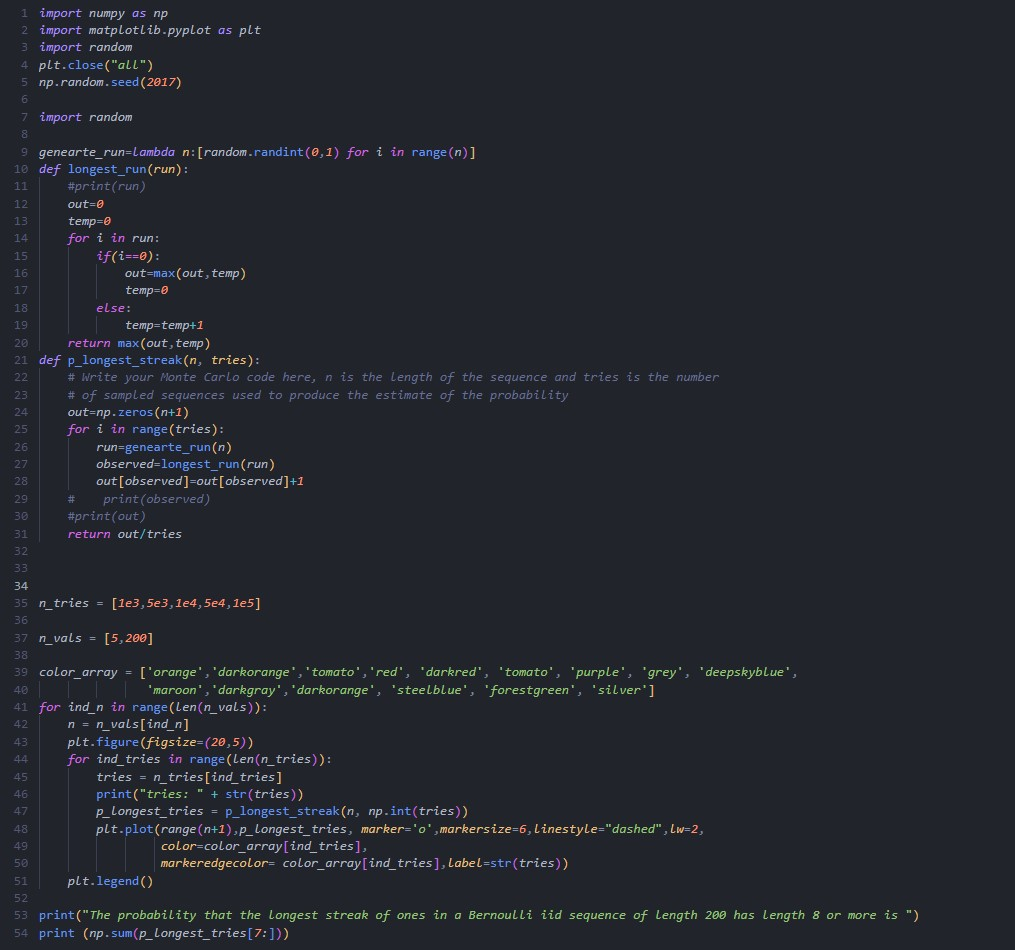
\includegraphics[width=15cm]{homework 1/50_badgers.jpg}
 \end{itemize}}
 \item What is the estimated probability that the longest streak of heads has length 8 or more for 200 flips? Is the sequence of 8 ones evidence that the program may not be generating truly random sequences?  
 \blue{
 \begin{itemize}
     \item the likelihood that there will be a run of 8 heads out of 200 flips is about $54\%$, this does seem to imply that it is more likely in a fair  program for there to be a sequence of 8 heads than for there not to be a sequence of 8 heads. So it is not evidence that the program is unfair. 
     \item 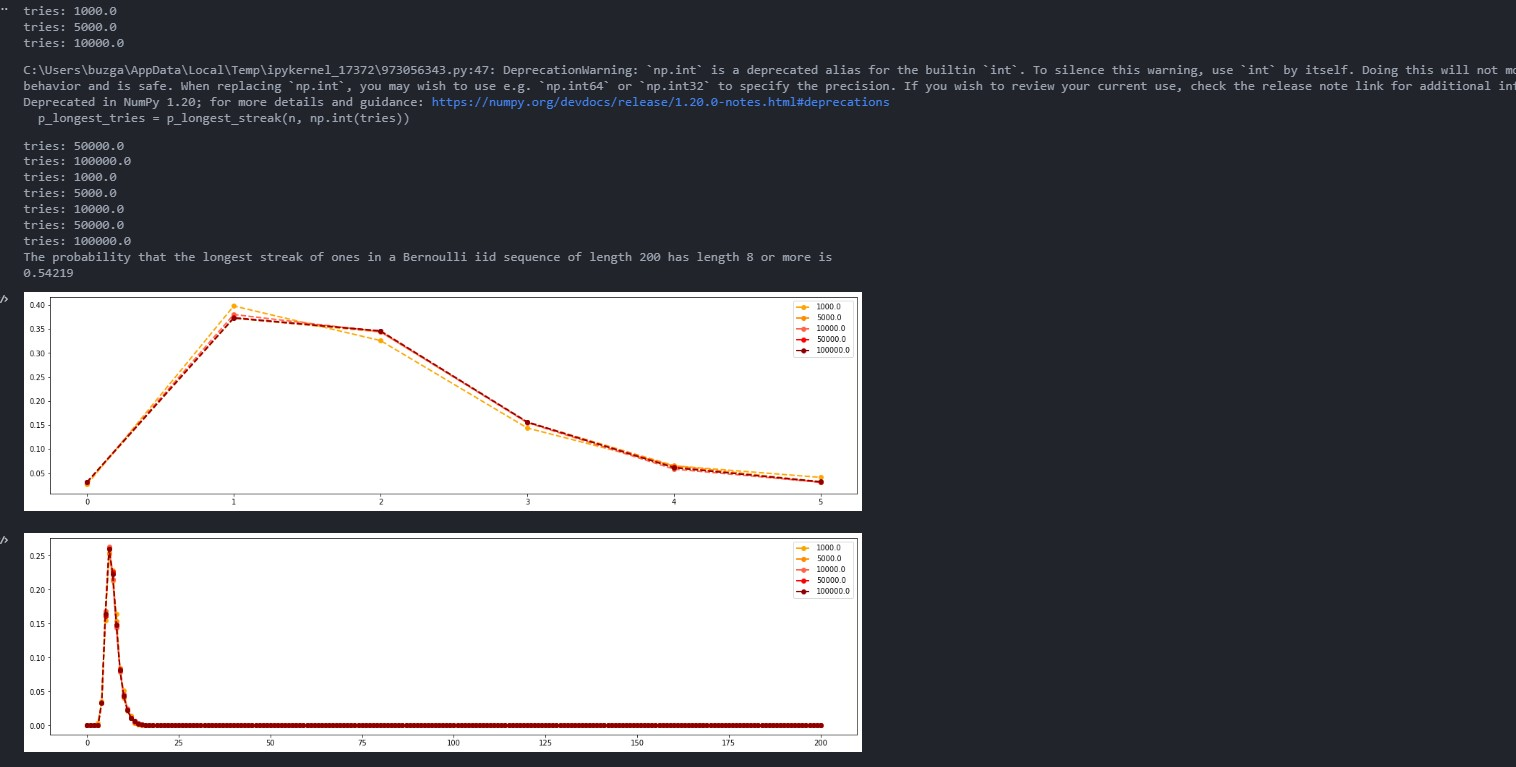
\includegraphics[width=15cm]{homework 1/50k_a_day.jpg}
 
 \end{itemize}
}
\end{enumerate}

\end{enumerate}
\end{document}
